\documentclass{standalone}
\usepackage{tikz}


\begin{document}

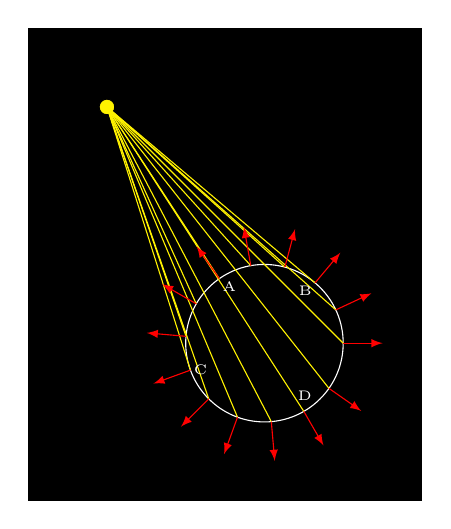
\begin{tikzpicture}
  \draw[fill=black] (-3,-2) rectangle (2,4);
  \draw[white] (0,0) circle [radius=1cm];

  \coordinate (light) at (-2,3);

  \draw[fill=yellow] (-2,3) circle [radius=0.1cm];

  \foreach \x in {0,25,...,345} {
    \draw[yellow] (light) -- (\x:1);
  }

  \foreach \x in {0,25,...,345} {
    \draw[-latex,red] (\x:1) -- (\x:1.5);
  }

  \node[white,anchor=north west,font=\tiny,inner sep=1pt] at (125:1) {A};
  \node[white,anchor=north east,font=\tiny,inner sep=1pt] at (50:1) {B};
  \node[white,anchor=west,font=\tiny,inner sep=1pt] at (200:1) {C};
  \node[white,anchor=south east,font=\tiny,inner sep=1pt] at (-50:1) {D};
\end{tikzpicture}

\end{document}